\documentclass[oneside]{article}
\usepackage{fullpage}
\usepackage[small]{titlesec}
\usepackage[pdftex]{graphicx}
\usepackage[round,sectionbib]{natbib}
\DeclareGraphicsExtensions{.png,.pdf}
\graphicspath{{examples/}}
% \usepackage{setspace} 
% \doublespacing

\begin{document}
\title{Two techniques for teaching inference: the statistical justice system and visual inference}
\author{Hadley Wickham, Heike Hofmann, Dianne Cook, Andreas Buja}
\date{13 May 2010}

\maketitle
\begin{abstract}

The statistical justice system makes hypothesis testing easier to understand and remember by connecting it to a concrete and familiar entity: the criminal justice system.

\end{abstract}

\section{Introduction}

Inference, testing and estimation, is one the most important aspects of statistics, yet it is one that students struggle to understand. This paper introduces two techniques that we have found helpful to give students metaphors to better understand how it works. 

This short note introduces the statistical justice system ({\sc sjs}), a fun and memorable metaphor for teaching hypothesis testing based on its similarity to the criminal justice system. Hypothesis testing is an important part of statistics, but students often struggle because of it is abstract and has convoluted terminology (e.g. fail to reject the null). The statistical justice system provides a concrete and familiar metaphor on which to pin new terminology. The idea of connecting hypothesis testing to the justice system is not new (wikipedia even mentions parts of it in the article on hypothesis testing), but we have not been able to find a published account that goes into complete detail.

Visual inference \citep{buja:2009,me:inf4info} is a rigorous alternative to classical inference, that uses the same principles, apart from two aspects: the test statistic, and the mechanism of computing similarity. The test statistic is now a plot of the data, and instead of a mathematical measurement of difference, we use a human judge, or even jury. Compared to graphics alone, visual inference offers a rigorous approach to avoid seeing pattern in noise,  and compared to purely mathematical inference it tests a much wider set of potentially interesting hypotheses.

Visual inference is useful for teaching inference because to start students just need to be able to recognise which plot is difference.  This makes concrete the ideas of the {\sc sjs} and helps students to build an understanding of what a null distribution (distribution of innocents) looks like.

\section{The statistical justice system}

A suspect (data set) is accused of a crime (having a particular parameter value) and is declared guilty or not guilty based on the results of a trial (statistical test). Each trial has a defence (advocating the null hypothesis) and a prosecution (advocating the alternative hypothesis). On the basis of how evidence (the test statistic) compares to a standard (the null distribution), the judge makes a decision to convict (reject the null) or acquit (fail to reject the null hypothesis).

In the {\sc sjs}, unlike in the criminal justice system, evidence is based on the similarity between the accused and known innocents. The population of innocents is called the null distribution and is generated by the combination of null hypothesis and test statistic. Typically, the level of guilt of the suspect is summarised with a single number, the proportion of true innocents who appear more guilty than they do. This is the $p$-value, the probability that a truly innocent person would look as (or more) guilty than the accused.  (We particularly like the description of the $p$-value in this metaphor - it's concrete and easy to understand.)

There are two types of mistakes we can make in our decision: we can falsely acquit a guilty dataset (a type II error, or false negative), or falsely convict an innocent dataset (a type I error, or false positive). Just as in the criminal justice system, the costs of these two mistakes are not equal and vary based on the severity of the consequences (the risk of letting a guilty shoplifter go free is not equal to the risk of letting a guilty axe-murderer go free). 

As in the criminal justice system, we can never prove that a suspect is innocent (absence of evidence is not evidence of absence). This is why a suspect is innocent until proven guilty, and why we fail to reject the null rather than accepting the alternative.

\section{Visual inference}
\label{sec:visual_inference}

The basic idea of visual inference is to (without looking at it first) embed the plot of the true data in a set of $n - 1$ null plots, plots of data from the null distribution. You then look at the panel of plots and pick the plot that is most unusual. If you correctly pick the true data as being different, then you have evidence ($p = 1/n$) that there is signal, and you are not just responding to random fluctuations.

To illustrate these ideas we'll use examples from classes that I taught, based on play-by-play data from Los Angeles Lakers games in the 2008 {\sc nba} season.

\subsection{Poisson, exponential and gamma distributions}
\label{sub:univariate}

Is the distribution of points scored by the Lakers a Poisson distribution?

\begin{figure}[htbp]
  \centering
    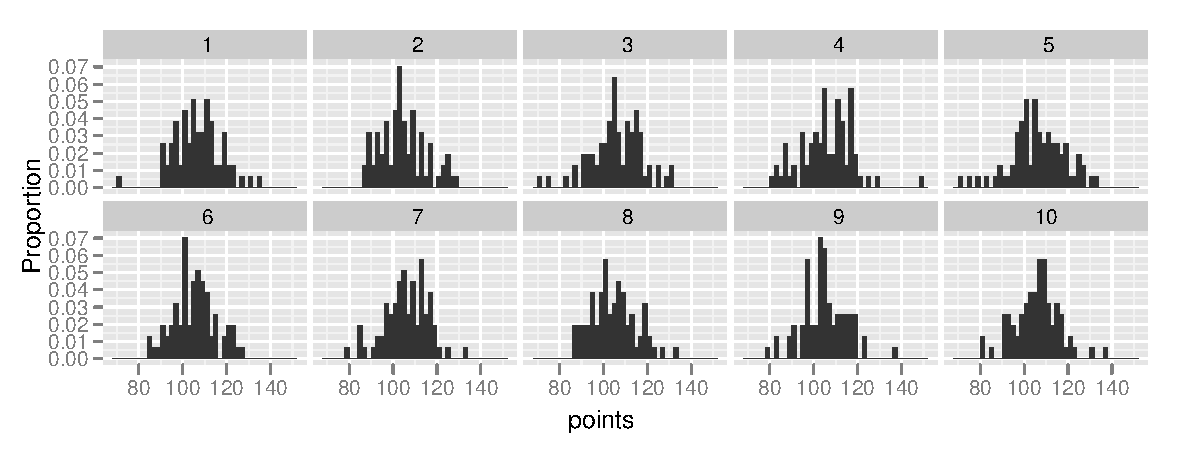
\includegraphics[width=\linewidth]{poisson}
  \caption{The distribution of points scored per game by the Lakers, hidden amongst nine plots generated under the null hypothesis of a Poisson distribution.}
  \label{fig:poisson}
\end{figure}

True data is in panel 3.

Compare this to plot that shows the data distribution overlaid with a theoretical distribution, Figure~\ref{fig:poisson-overlay}

\begin{figure}[htbp]
  \centering
    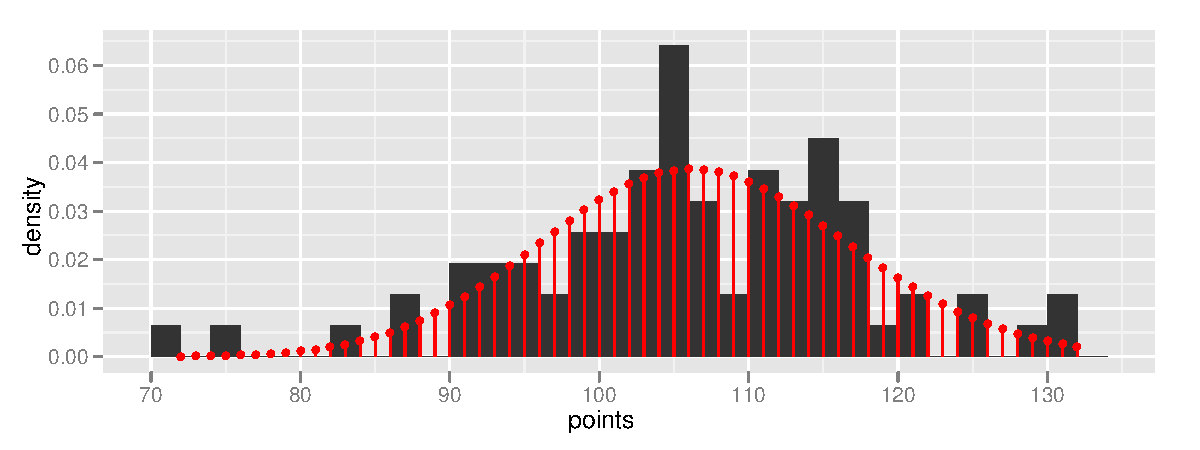
\includegraphics[width=0.5\linewidth]{poisson-overlay}
  \caption{Data overlaid with theoretical pdf in red.}
  \label{fig:poisson-overlay}
\end{figure}

We know that if the distribution of waiting times is exponential, then the distribution of counts in a fixed time will be Poisson.  What does the distribution of waiting times between points look like? Figure~\ref{fig:exponential} shows the distribution from the data hidden amongst 9 null plots generated from an exponential distribution with parameters matched to the data.

\begin{figure}[htbp]
  \centering
    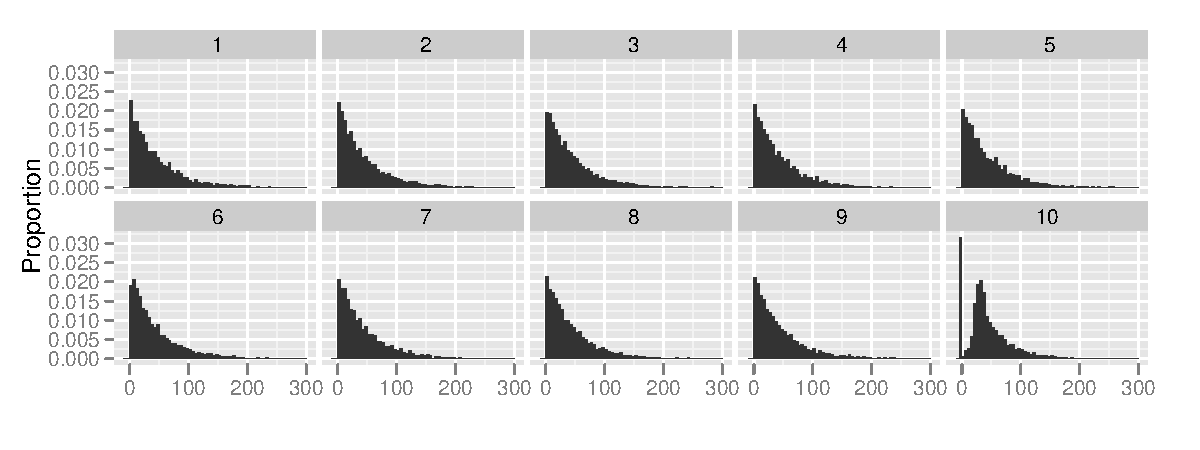
\includegraphics[width=\linewidth]{exponential}
  \caption{The distribution of waiting times between points, hidden amongst nine plots generated under the null hypothesis of a exponential distribution.}
  \label{fig:exponential}
\end{figure}

The true data (in panel 10) is strikingly obvious: there are a large number of waiting times that are 0. These represent free throws and other penalties when the game clock is stopped. Figure~\ref{fig:gamma} removes free throws, focussing only on the waiting time between field goals, and for the null plots uses the slightly more flexible gamma distribution. Can you spot the true data?

\begin{figure}[htbp]
  \centering
    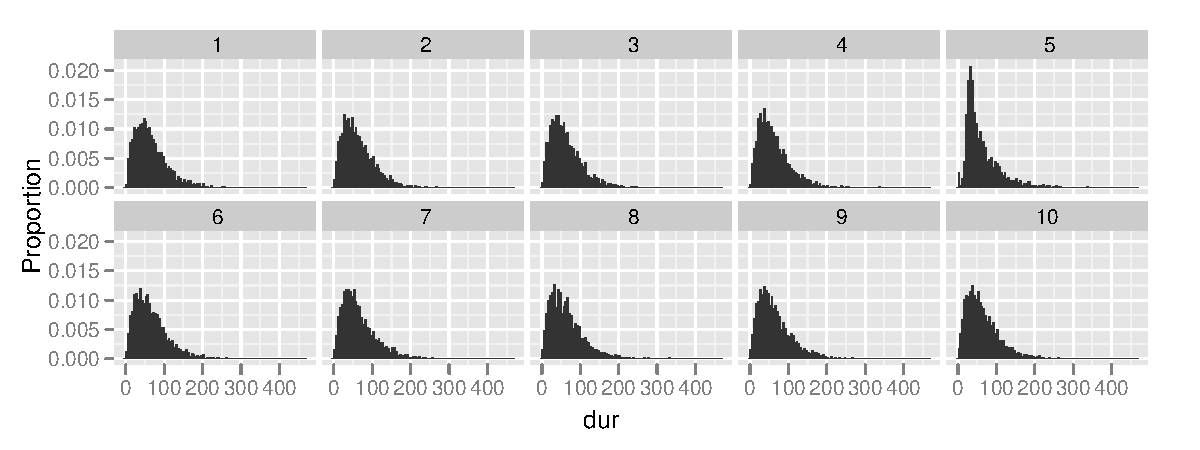
\includegraphics[width=\linewidth]{gamma}
  \caption{The distribution of waiting times between field goals, hidden amongst nine plots generated under the null hypothesis of a gamma distribution.}
  \label{fig:gamma}
\end{figure}

The true data is in panel 5, thus we have evidence to reject the hypothesis that the points are distributed randomly.  This is unfortunate because the parameters of the gamma have a nice interpretation here: the rate of shot attempts is 28 seconds, and on average, 1 in 2.3 are successful.

\subsection{Scatterplots}
\label{sub:bivariate}


\section{Conclusions}

I used this presentation of hypothesis testing in class this year. Anecdotally, it seemed to help students better understand testing. The connection between the arguments of the defence and the null hypothesis helped them correctly identify the null in problems. The description of the $p$-value as the probability an innocent would look this guilty, seemed to help to avoid some of the common misinterpretations.

Students liked this presentation of the material and in the end of semester reviews, 5 out of 43 said that it was their favourite lecture of the semester. This is pretty impressive for a lecture on hypothesis testing!

% bibtool -x sjs.aux > references.bib
\bibliography{references}
\end{document}
